\section*{Arrival Functions}
Three models are considered in this section, a staircase, an affine, and a linear model as seen on \autoref{fig:arrivalCurves}. The staircase and affine models are used to approximate the real unknown arrival function, while the linear model is a service curve showing the capabilities of the network.\\

The staircase arrival model in relation to the real unknown arrival function is given by
\begin{flalign}
  R(t) \leq Sc(t) &= \left\lceil \frac{t - \mathrm{offset}}{T} \right\rceil \times P \ \ ,&
\end{flalign}
%
\begin{where}
  \va{R(t)}{is the real unknown arrival curve.}{}
  \va{Sc(t)}{is the staircase model arrival curve for the wheel sensor data.}{}
  \va{t}{is the time.}{}
  \va{\mathrm{offset}}{is the time offset measured from $t = 0$ to first packet arrival.}{}
  \va{T}{is the period time for packet arrivals.}{}
  \va{P}{is the packet size.}{}
\end{where}

The worst case is when the offset goes to zero, this means that a packet arrives at time zero.

\begin{figure}[H]
  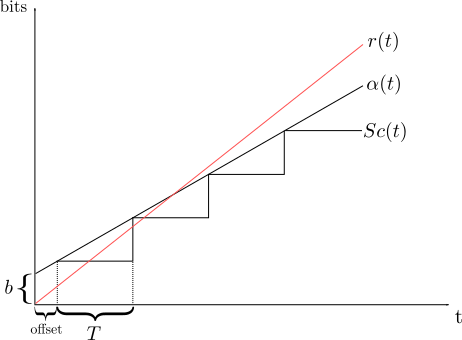
\includegraphics[width = .4\textwidth]{arrivalCurves}
  \caption{$Sc(t)$ is the staircase arrival curve, $\alpha(t)$ is the affine model arrival curve and $r(t)$ is the service curve defined by the capabilities of the CAN Bus.}
  \label{fig:arrivalCurves}
\end{figure}

The affine arrival model in relation to the real unknown arrival function is given by
\begin{flalign}
  R(t) \leq \alpha (t) &= b + \frac{P}{T} t &
\end{flalign}
%
\begin{where}
  \va{\alpha}{is the affine model arrival curve}{}
  \va{b}{is the crossing of the affine curve with the y-axis}{}
\end{where}
%
The relation between both models and the unknown real arrival function is then given by
\begin{flalign}
  R &\leq Sc \leq \alpha &
\end{flalign}

\subsection{Wheel Sensor Data Arrival}
The staircase arrival model for the wheel sensor data is
\begin{flalign}
  Sc_\mathrm{w} (t) &= \left\lceil \frac{t - \cancelto{0}{\mathrm{offset}} \ \ \ }{T_\mathrm{w}} \right\rceil \times P_\mathrm{w}& \\
  Sc_\mathrm{w} (t) &= \left\lceil \frac{t}{0.04} \right\rceil \times 160 \ \ ,&
\end{flalign}
where $P_\mathrm{w} = 20\times 8$ since the packet size is \SI{20}{B}, which means that \SI{160}{b} arrive at each time interval, $T = 0.04$. The time offset is set to zero in order to model for worst case.
%
%\begin{where}
%  \va{Sc_\mathrm{w} (t)}{is the staircase model arrival curve for the wheel sensor data.}{}
%  \va{t}{is the time.}{}
%  \va{\mathrm{offset}}{is the time offset measured from $t = 0$ to first packet arrival.}{}
%  \va{T_\mathrm{w}}{is the period time for packet arrivals from the wheel sensors.}{}
%  \va{P_\mathrm{w}}{is the packet size containing the wheel sensor data.}{}
%\end{where}
%
%
The affine arrival model for the wheel sensor data is
\begin{flalign}
  \alpha_\mathrm{w} (t) &= b + \frac{P_\mathrm{w}}{T_\mathrm{w}} t & \\
  \alpha_\mathrm{w} (t) &= 160 + \frac{160}{0.04} t  = 160 + 6.4 t \ \ ,&
\end{flalign}
where $b = P_\mathrm{w} = 160$ since the time offset is set to zero to model worst case.
%
%\begin{where}
%  \va{\alpha_\mathrm{w} (t)}{is the affine model arrival curve for the wheel sensor data}{}
%  \va{b}{is the crossing of the affine curve with the y-axis}{}
%\end{where}
%
%

\subsection{Electronic Speed Control (ESC) Data Arrival}
The staircase arrival model for the wheel sensor data is
\begin{flalign}
  Sc_\mathrm{ESC} (t) &= \left\lceil \frac{t - \cancelto{0}{\mathrm{offset}} \ \ \ }{T_\mathrm{ESC}} \right\rceil \times P_\mathrm{ESC}& \\
  Sc_\mathrm{ESC} (t) &= \left\lceil \frac{t}{0.4} \right\rceil \times 64 \ \ ,&
\end{flalign}
where $P_\mathrm{ESC} = 8\times 8$ since the packet size is \SI{8}{B}, which means that \SI{64}{b} arrive at each time interval, $T = 0.4$. The time offset is again set to zero in order to model for worst case.
%
%\begin{where}
%  \va{Sc_\mathrm{w} (t)}{is the staircase model arrival curve for the wheel sensor data.}{}
%  \va{t}{is the time.}{}
%  \va{\mathrm{offset}}{is the time offset measured from $t = 0$ to first packet arrival.}{}
%  \va{T_\mathrm{w}}{is the period time for packet arrivals from the wheel sensors.}{}
%  \va{P_\mathrm{w}}{is the packet size containing the wheel sensor data.}{}
%\end{where}
%
The affine arrival model for the wheel sensor data is
\begin{flalign}
  \alpha_\mathrm{ESC} (t) &= b + \frac{P_\mathrm{ESC}}{T_\mathrm{ESC}} t & \\
  \alpha_\mathrm{ESC} (t) &= 64 + \frac{64}{0.4} t = 64 + 25.6 t \ \ ,&
\end{flalign}
where $b = P_\mathrm{ESC} = 64$ since the time offset is set to zero to model worst case.

\begin{figure}[H]
	\captionbox
	{
		Arrival curves for the four wheels and service curve for the CAN-bus.
		\label{fig:ArrivalCurvesWheels}
	}
	{
		\includegraphics[width=.46\textwidth]{figures/ArrivalCurvesWheels}
	}
	\hspace{5pt}
	\captionbox
	{
		Arrival curves for the ESC and service curve for the CAN-bus.
		\label{fig:ArrivalCurvesESC}
	}
	{
		\includegraphics[width=.46\textwidth]{figures/ArrivalCurvesESC}
	}
\end{figure}
\section{Token Filter}

\begin{figure}[H]
	\includegraphics[width = .4\textwidth]{tokenFilter}
	\caption{Token filter}
	\label{fig:tokenFilter}
\end{figure}
%
\begin{figure}[H]
	\captionbox
	{
		Arrival curves for the Multimedia and service curve for the CAN-bus.
		\label{fig:ArrivalCurvesMultimedia}
	}
	{
		\includegraphics[width=.46\textwidth]{figures/ArrivalCurvesMultimedia}
	}
	\hspace{5pt}
	\captionbox
	{
		Arrival curves for the RC and service curve for the CAN-bus.
		\label{fig:ArrivalCurvesRC}
	}
	{
		\includegraphics[width=.46\textwidth]{figures/ArrivalCurvesRC}
	}
\end{figure}
%
\subsection{Service Model}
The curve for the service model, $r(t)$, is seen in \autoref{fig:arrivalCurves}. The model is linear and defined by the capabilities of the CAN Bus with a rate of \SI{1}{Mbps}.


\section{Reliability}
The failure rate can be translated to be in fails/year. This is done in \autoref{eq:failrate}.

\begin{flalign}
	\lambda=\frac{1 \mathrm{fails}}{2\cdot10^6\mathrm{h}}\cdot\frac{8760 \mathrm{h}}{1\mathrm{year}}=\frac{1 \mathrm{fails}}{288.3\mathrm{year}}
	\label{eq:failrate}
\end{flalign}

The lifetime of the car can be expressed by its probability density function seen in \autoref{eq:carpdf}.
\begin{flalign}
	f_{\mathrm{car}}(t)=
	\begin{cases}
		\frac{1}{10} & \text{if } t\in[5,15]\\
		0               & \text{otherwise}
	\end{cases}
	\label{eq:carpdf}
\end{flalign}
\subsection{Case 1}
For the first case, the reliability, cumulative and probability functions for the lifetime of the network can be found. The first one obtained is the reliability function and it is found by multiplying the individual reliabilities for the two switches as they are connected in series, see \autoref{fig:case1}, and they have independent probabilities of failing. 
\begin{figure}[H]
	\includegraphics[width = .2\textwidth]{case1}
	\caption{Switch diagram for case 1}
	\label{fig:case1}
\end{figure}

\begin{flalign}
	R_{\mathrm{n}}(t)&=R_1(t)R_2(t)=e^{-\lambda t}e^{-\lambda t}=e^{-2\lambda  t}\label{eq:reliabilitycase1} \\
	F_{\mathrm{n}}(t)&=1-R_{\mathrm{n}}(t)=1-e^{-2\lambda t} \label{eq:cumulativecase1}  \\
	f_{\mathrm{n}}(t)&={F^{\prime}}_{\mathrm{n}}=-2 \lambda e^{{-2\lambda t}} \label{eq:probabilitycase1}  
\end{flalign}

To find the probability of the network failing before the rest of the car does, a double integration is performed from 5 to 15 for and from 0 to $t_{\mathrm{c}}$, where $t_{\mathrm{c}}$ is the time in which the car fails. \autoref{eq:integralcase1} shows the performed computation.


\begin{flalign}
	P(t_\mathrm{n}-t_\mathrm{c})&=\int_{5}^{15}\left[\int_{0}^{t_{\mathrm{c}}}f_{\mathrm{n}}(t)f_{\mathrm{c}}(t)dt_{\mathrm{n}}\right]dt_{\mathrm{c}}\label{eq:integralcase1}
\end{flalign}

The result of this integral gave a probability of 0.0668 of the network failing before the rest of the car.
\subsection{Case 2 a}
In case 2 a, one of the switches is duplicated as seen in \autoref{fig:case2a}. Even though the method is the same, the reliability, cumulative and probability functions change as now there is one more switch in the network. 
\begin{figure}[H]
	\includegraphics[width = .4\textwidth]{case2a}
	\caption{Switch diagram for case 2 a}
	\label{fig:case2a}
\end{figure}
\begin{flalign}
	R_{\mathrm{n}}(t)&=R_2(R_1(t)+R_3(t)-R_1(t)R_3(t))=e^{-\lambda t}\left(2e^{-\lambda t}-e^{-2\lambda  t}\right)= 2e^{-2\lambda  t} - e^{-3 \lambda t} \label{eq:reliabilitycase2a} \\
	F_{\mathrm{n}}(t)&=1-R_{\mathrm{n}}(t)= 1-2e^{-2\lambda  t} + e^{-3 \lambda t}\label{eq:cumulativecase2a}  \\
	f_{\mathrm{n}}(t)&={F^{\prime}}_{\mathrm{n}}=4 \lambda e^{{-2\lambda t}} -3 \lambda e^{{-3\lambda t}}  \label{eq:probabilitycase2a}  
\end{flalign}

The integral is done in the same way as seen in \autoref{eq:integralcase1} but in this case the expression for $f_{\mathrm{n}}$ is different. The result obtained is 0.00346.

\subsection{Case 2 b}
In the last case, both switches are duplicated. The structure is shown in \autoref{fig:case2b}. Again, the reliability, cumulative and probability functions change and they need to be re-calculated taking into account the new combination of series and parallel connection. This is shown in \autoref{eq:reliabilitycase2b} and \ref{eq:cumulativecase2b} and \ref{eq:probabilitycase2b}.
\begin{figure}[H]
	\includegraphics[width = .4\textwidth]{case2b}
	\caption{Switch diagram for case 2 b}
	\label{fig:case2b}
\end{figure}
\begin{flalign}
	R_{\mathrm{n}}(t)&=(R_1(t)+R_3(t)-R_1(t)R_2(t))(R_2(t)+R_4(t)-R_2(t)R_4(t))=\label{eq:reliabilitycase2b} \\
			&\left(2e^{-\lambda t}-e^{-2\lambda  t}\right)\left(2e^{-\lambda t}-e^{-2\lambda  t}\right)=\left(4e^{-2\lambda t}-4e^{-3\lambda t}+e^{-4\lambda t}\right)\nonumber\\
	F_{\mathrm{n}}(t)&=1-R_{\mathrm{n}}(t)=1-e^{-2\lambda t} \label{eq:cumulativecase2b}  \\
	f_{\mathrm{n}}(t)&={F^{\prime}}_{\mathrm{n}}=-2 \lambda e^{{-2\lambda t}} \label{eq:probabilitycase2b}  
\end{flalign}

The new probability density function is used to find the probability of the network failing before the car does in the same way as with the previous two cases. See \autoref{eq:integralcase1}. The result obtained for this case is 0.0025. 

It can be seen that the failure probability is reduces the more redundant components are present in the network.
